% A typical 1-cocycle: each 1-simplex is labeled with its assigned value,
% arranged so that every cycle sums to 0.
% Source: book/tex/homology/cohomology.tex (§ Visualization of cohomology groups).
\documentclass[border=2mm]{standalone}
\usepackage{tikz}
\usepackage{amssymb}
\usetikzlibrary{arrows.meta}
\begin{document}
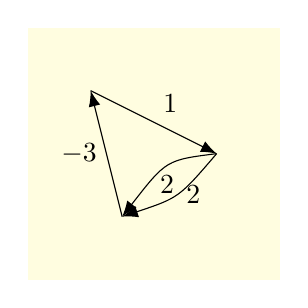
\begin{tikzpicture}[scale=0.8, >={Latex[length=2mm]}]
  \fill[yellow!12] (0,0) rectangle (4,4);
  \draw[->] (1.5,1) -- (1,3) node[midway, left] {$-3$};
  \draw[->] (1,3) -- (3,2) node[midway, above right] {$1$};
  \draw[->] (3,2) .. controls (2.2,1.9) .. (1.5,1) node[midway, below] {$2$};
  \draw[->] (3,2) .. controls (2.4,1.3) .. (1.5,1) node[midway, right] {$2$};
\end{tikzpicture}
\end{document}
